\section{The Standard Model}

\label{sec:SM}
\subsection{Overview}
\label{subsec:Overview}
The Standard Model (SM) of particle physics is a mathematical framework based on quantum field theory which incorporates quantum mechanics and special relativity and describes the known fundamental particles in nature and all their interactions. It consists of two sets of particles with intrinsic angular momentum, half-integer-spin fermions which are fundamental constituents of matter particles, and force-carrying integer-spin bosons. The seventeen fundamental particles of the SM and their properties such as mass, charge, and intrinsic spin are shown schematically by figure \ref{fig:SM}. Discussion in this section is written with the guidance from three textbooks of particles, Mark Thomson's Modern Particle Physics \cite{Thomson:2013zua}, and Halzen $\&$ Martin's Quarks $\&$ Leptons \cite{Halzen:1984mc}.

\begin{figure}[H]
	\centering
    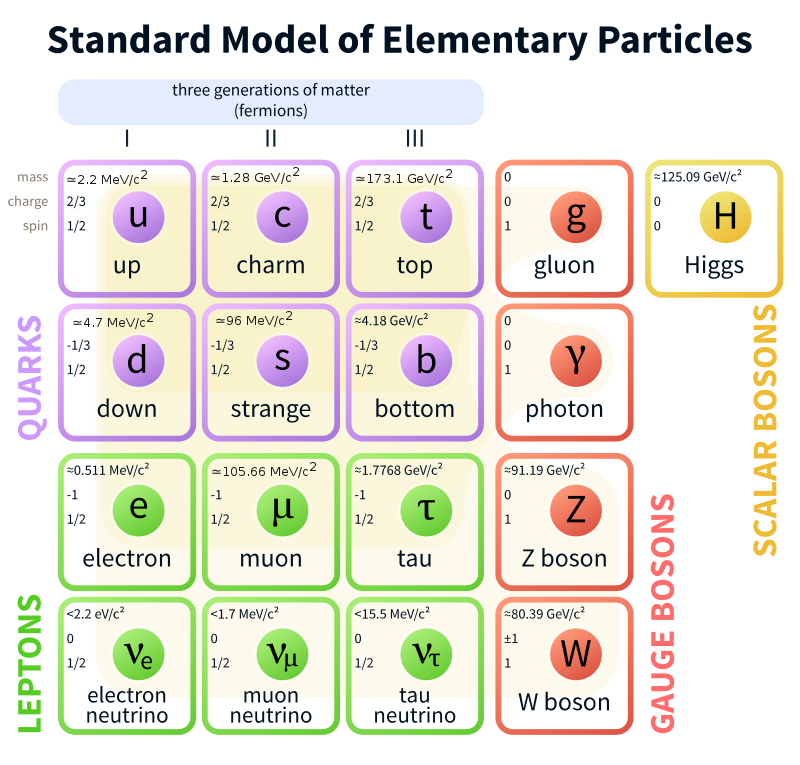
\includegraphics[width=0.7\textwidth] {figures/SMparticles.png}\hspace{1cm}
    \caption{ The seventeen fundamental particles of the Standard Model include three generations of twelve fermions, four gauge bosons, and the scalar Higgs bosons. \cite{SMFigureWiki}}
    \label{fig:SM}
\end{figure}

The twelve half-integer-spin fermions can be further distinguished into two categories, leptons, and quarks, each having three generations of particles with similar properties as shown schematically by figure \ref{fig:SM}. For each fermion, there exists an anti-fermion with the same additive quantum numbers but with opposite signs. The four spin $1$ bosons shown in Table \ref{tab:VectorBosons} are collectively called the gauge bosons. The quanta of these gauge fields mediate the electromagnetic, weak, and strong interactions. Gauge fields are invariant under various local group transformations that preserve some quantum numbers associated with the interactions and are discussed in detail in Section \ref{subsec:TheoryFormulation} \cite{Bernabeu2021}. Different fermions take part in different interactions as outlined by Table \ref{tab:FermionInteraction}, and the strength of the interaction is governed by a gauge coupling parameter.

Massless photon ($\gamma$) mediates the electromagnetic interaction. The massive $W$ and $Z$ bosons mediate weak interaction. The Standard Model unifies electromagnetic and weak forces to a unified electroweak theory which follows from $SU(2)_{L}~\otimes~U(1)_{Y}$ gauge symmetry discussed in detail in Section \ref{subsubsec:EWkUni}. Weak isospin (I) and weak hypercharge (Y) are the quantum numbers associated with the $SU(2)_{L}$ and $U(1)_{Y}$ gauge groups respectively. The electric charge (Q) which is conserved in all interactions is related to the isospin and hypercharge by $Q=I_3 + \frac{Y}{2}$, where $I_3$ is the third component of the weak isospin. The $SU(2)_{L}$ group follows a chiral structure where the gauge fields couple explicitly to the left-handed (LH) chiral fermions states and the right-handed (RH) chiral anti-fermions states. Thus, each generation of fermion contains a left-handed doublet with $I=\frac{1}{2}$ and a right-handed singlet carrying $I=0$ which are shown in Table \ref{tab:Fermions}. 

\begin{table}
\caption{Properties of Standard Model gauge bosons.\cite{PDG}}
\begin{center}
\begin{tabular}{| c | c | c | c | c | c |}
\hline
\multicolumn{2}{|c|}{Interaction Type }	& Particle 		          & 	Q 		& 	Mass $[GeV]$ 		& Symmetry Group \\ 
\hline
\multirow{3}{*} {Electroweak}  & Electromagnetic 		& Photon ($\gamma$)      &   	   0                    & 	$0$	 			&  \multirow{3}{*}{$SU(2)~\otimes~U(1)$}		\\
					      &  \multirow{2}{*} { Weak }          		& $W^{\pm}$	&   $\pm1$	&	$80.4$	&		\\
    	  				       &	  &	$Z$ boson  			& $0$ 		    	         & 	          $91.2$			&   		  \\
\hline
\multicolumn{2}{|c|}{Strong } & gluons (g) &  0 & 0 & $SU(3)$ \\
\hline 
\end{tabular}
\label{tab:VectorBosons}
\end{center}
\end{table}

\begin{table}
\caption{ Summary of different interactions of fermions under different gauge theory. The check mark suggest that the fermions interact via associated force.}
\begin{center}
\begin{tabular}{| c | c | c |  c | c |}
\hline
\multicolumn{2}{|c|} {Particles} & Strong $SU(S)$ & Electromagnetic $U(1)$ & Weak $SU(2)$ \\
\hline
\hline
\multirow{2}{*} {Quarks} & $u, c, t$ &  \multirow{2}{*} \checkmark & \multirow{2}{*} \checkmark & \multirow{2}{*} \checkmark \\
  & d, s, b &  & &\\
\hline
\multirow{2}{*} {Leptons} & e, $\mu$, $\tau$ &  - &  \checkmark &  \checkmark \\
 & $\nu_{e}$, $\nu_{\mu}$, $\nu_{\tau}$ & - & \checkmark & - \\
\hline
\end{tabular}
\label{tab:FermionInteraction}
\end{center}
\end{table}

Each generation of lepton, electron $(e)$, muon $(\mu)$ and tau $(\tau)$ is accompanied by a neutral particle called neutrino $(\nu)$ with same lepton flavor $(\nu_e, \nu_{\mu} \& \nu_{\tau})$. The lepton flavor is conserved by the Standard Model. Standard Model neutrinos are their own anti-particles and only left-handed neutrinos are predicted by the theory.

The quarks can be further categorized into two categories, the up-type quarks with $+\frac{2}{3}$ charge and the down-type quarks with $-\frac{1}{3}$ charge. Up $(u)$, charm  $(c)~,~\&$ top $(t)$ are the first, second, and third generation of the up-type quarks, while the down $(d)$, strange $(s)$ $\&$ bottom $(b)$ are the three generations of the down-type quarks. The down-type left-handed quarks in $SU(2)_{L}$ quark doublets $d^{'},~s^{'}~ \&~b^{'}$ summarized in table \ref{tab:Fermions} are linear combinations of $d,~s,~b$ quarks. The quarks interact strongly with one another by strong interaction mediated by the massless neutral gluons which follow from $SU(3)$ gauge symmetry by exchange of color charges. Each quark can have either one of the three color charges (red, blue $\&$, green), whereas an anti-quark can have either anti-red, anti-blue, or anti-green color charge. There are eight gluons in the Standard Model with color charges formed by a combination of either of the two color charges. Since gluons have a color charge, they interact with other gluons strongly. 

\begin{table}
\caption{Electroweak quantum numbers of Standard Model half-integer spin fermions (quarks and leptons) arranged in a left-handed $SU(2)$ doublet and right-handed $SU(2)$ singlet.\cite{Halzen:1984mc}}
\begin{center}
\begin{tabular}{| c | c | c | c | c | c | c |}
\hline
{Particle Types }			& First		& Second	&   Third        & 	$I_{3}$ 	& Y & Q  \\ 
\hline
\hline					
\multirow{5}{*} {Leptons}  	
	& & & & & & \\
					& $\begin{pmatrix}  e \\ \nu_{e} \end{pmatrix}_{L}$ 
					& $\begin{pmatrix}  \mu \\ \nu_{\mu} \end{pmatrix}_{L}$
					& $\begin{pmatrix}  \tau \\ \nu_{\tau} \end{pmatrix}_{L}$  
					& $\begin{matrix} -\frac{1}{2} \\[0.15cm] \frac{1}{2} \end{matrix}$ 
					& $\begin{matrix} -1 \\ -1 \end{matrix}$   
					& $\begin{matrix} -1 \\ 0 \end{matrix}$ \\		
	& & & & & & 	\\				
					& $e_{R}$ & $\mu_{R}$ &  $\tau_{R}$ & $0$ & $-2$  & $-1$ \\
\hline
\hline
\multirow{8}{*} {	Quarks}  	
& & & & & & \\
					 &$\begin{pmatrix}  u \\ d^{'} \end{pmatrix}_{L}$ 
					 &$\begin{pmatrix}  c \\ s^{'} \end{pmatrix}_{L}$
					 &$\begin{pmatrix}  t \\ b{'} \end{pmatrix}_{L}$  
					&$\begin{matrix} \frac{1}{2} \\[0.15cm] -\frac{1}{2} \end{matrix}$
					&$\begin{matrix} \frac{1}{3} \\[0.15cm] \frac{1}{3} \end{matrix}$
					&$\begin{matrix} \frac{2}{3} \\[0.15cm] -\frac{1}{3} \end{matrix}$\\
				& & & & & & \\
					& $u_{R}$ & $c_{R}$ &  $t_{R}$ & $0$ & $\frac{4}{3}$  & $\frac{2}{3}$ \\
					& & & & & & \\
					& $d_{R}$ & $s_{R}$ &  $b_{R}$ & $0$ & $-\frac{2}{3}$  & $-\frac{1}{3}$ \\
& & & & & & \\
\hline
\end{tabular}
\label{tab:Fermions}
\end{center}
\end{table}

Higgs boson is the only spin-0 scalar particle in the theory with no charge and gives masses to all other particles through Spontaneous Symmetry Breaking which will be discussed in section \ref{subsubsec:EWkUni}.

\subsection{Theoretical Formulation of the Standard Model}
\label{subsec:TheoryFormulation}
I guess the best way to organize this sub section would be to discuss the following bullet points in detail.
\begin{itemize}
\item{motivate QFT}
\item{introduce fields and Dirac spinors??}
\item{fermion,gauge,scalar fields introduction? }
\end{itemize}

\subsubsection{Relativistic Quantum Field Theory}
\label{subsubsec:RelQFT}
Relativistic quantum field theory is the theoretical framework that describes the elementary particles and their interactions of the Standard Model. This section introduces the framework. 

\subsubsection{Lagrangian of the Standard Model}
\label{subsubsec:SMLag}
The dynamics of the SM can be described by the Lagrangian density given in equation \ref{eqn:SMLagrangian} which is invariant under the local gauge transformation of the $SU(3)~\otimes~SU(2)_{L}~\otimes~U(1)_{Y}$ symmetry group. 

\begin{equation}
\mathcal{L_{SM}} = -\frac{1}{4}F_{\mu\nu}F^{\mu\nu} ~+~ i\bar{\psi}\gamma^{\mu}D_{\mu}\psi ~+~ |D_{\mu}\phi|^{2} ~+~ -V(\phi) + \bar{\psi_{i}}y_{ij}\psi_{j}\phi ~+~ h.c.
\label{eqn:SMLagrangian}
\end{equation}

The first term $-\frac{1}{4}F_{\mu\nu}F^{\mu\nu}$ describes the dynamics of the gauge boson interactions, the second term $i\bar{\psi}\gamma^{\mu}D_{\mu}\psi$ describes the interaction of the fermion fields. The third term $|D_{\mu}\phi|^{2}$ describes the couplings between the Higgs boson and gauge bosons, whereas the term $V(\phi)$ describes the Higgs potential and its self-interactions. The second last term $\bar{\psi_{i}}y_{ij}\psi_{j}\phi$ generates masses for fermions based on their Yukawa couplings $y_{ij}$ to the Higgs field. Similarly, the last term $h.c.$ generates masses for antifermions. 

SM respects the Poincar\'e symmetry making the Lagrangian in equation \ref{eqn:SMLagrangian} invariant under spacetime translations, rotations and boosts. The Lagrangian is also invariant under $SU(3)~\otimes~SU(2)_{L}~\otimes~U(1)_{Y}$ gauge transformations. According to Noether's theorem, a quantity is conserved for each continuous transformation that leaves the Lagrangian invariant. All three parts of the Standard Model, quantum electrodynamics (QED), quantum chromodynamics (QCD) and electroweak (EWK) are gauge theories whose Lagrangians are derived independently in sections below.

\subsubsection{Quantum Electrodynamics}
\label{subsubsec:QED}
Quantum electrodynamics describes the electromagnetic interaction. The Lagrangian density ($\mathcal{L}_{Dirac}$) describes the free propagation of a fermion in vacuum as:  

\begin{equation}
\mathcal{L}_{Dirac} = \bar{\psi} i \gamma^{\mu} \partial_{\mu} \psi ~-~ m\bar{\psi}\psi
\label{eqn:DiracLag}
\end{equation},

where $\psi$ is the fermionic spinor, $\gamma^{\mu}$ represents the Dirac matrices with $\mu$ being the Lorentz index running from $0$ to $3$, $\partial^{\mu}$ is the covariant derivative and m is the mass of the fermion \cite{}. 

The Lagrangian in equation \ref{eqn:DiracLag} is invariant under a $U(1)$ global gauge transformation, 
\begin{equation}
\psi\rightarrow \psi^{'}=e^{iq\alpha}\psi, 
\label{eqn:QEDGlobalTrans}
\end{equation}

where q is a parameter of the transformation itself and $\alpha$ is a real phase factor. However, under the local gauge transformation of form 

\begin{equation}
\psi\rightarrow \psi^{'}=e^{iq\alpha(x)}\psi
\label{eqn:QEDLocalTrans}
\end{equation}

which depends on $x~=~(x_{0},x_{1},x_{2},t)$ the Dirac Lagrangian in equation \ref{eqn:DiracLag} is not invariant. 

To make the Lagrangian of equation \ref{eqn:DiracLag} invariant, a gauge field $A_{\mu}$ is introduces with the following transformation properties, 

\begin{equation}
A_{\mu}\rightarrow A_{\mu} - \partial _{\mu} \alpha
\label{eqn:QEDGaugeField}
\end{equation}  

The $A_{\mu}$ couples to fermionic fields $\psi(x,t)$ with strength q. A covariant derivative specific to the local gauge transformation is defined as:

\begin{equation}
D_{\mu} = \partial_{\mu} - iqA_{\mu}
\label{eqn:QEDCovDerv}
\end{equation}  

The quantity $q$ can be interpreted as the electric charge $-e$ of fermion which gives the coupling strength of QED. With these substitutions the Dirac Lagrangian in equation \ref{eqn:DiracLag} changes to following

\begin{equation}
\mathcal{L} = \bar{\psi} ( i \gamma^{\mu} D_{\mu} ~-~ m) \psi = \bar{\psi} ( i \gamma^{\mu} \partial_{\mu} ~-~ m) \psi + e\bar{\psi} \gamma^{\mu} \psi A_{\mu}
\label{eqn:QEDInvLag}
\end{equation},

which is invariant under $U(1)$ gauge transformation respecting the $U(1)$ gauge symmetry. 

The gauge field $A_{\mu}$ can be interpreted as the photon field and is related to the electromagnetic field tensor by

\begin{equation}
F_{\mu\nu} = \partial_{\mu}A_{\nu} - \partial_{\nu}A_{\mu}
\label{QEDFieldTensor}
\end{equation}

The gauge invariant kinetic term of photon $-\frac{1}{4}F_{\mu\nu}F^{\mu\nu}$ can be inserted into the Lagrangian in equation \ref{eqn:QEDInvLag} which gives us the full Lagrangian of QED invariant under $U(1)$ gauge transformation. 

\begin{equation}
\mathcal{L}_{QED} = -\frac{1}{4}F_{\mu\nu}F^{\mu\nu} + \bar{\psi} ( i \gamma^{\mu} D_{\mu} ~-~ m) \psi
\label{eqn:QEDFullLag}
\end{equation}

$\mathcal{L}_{QED}$ in equation \ref{eqn:QEDFullLag} is the full Lagrangian for QED and the electromagnetic phenomena can be derived by solving for the equations of motion applying the Lorentz gauge condition $\partial_{\mu}A^{\mu}=0$. 
\textcolor{red}{maybe i add more description here on QED coupling constant?}

% dimensionless coupling constant ($\alpha_{QED}$) of QED as $\alpha_{QED} = \frac{e^2}{4\pi}$. \textcolor{red}{ 

\subsubsection{Quantum Chromodynamics }
\label{subsubsec:QCD}

\subsubsection{Electroweak Unification and the Higgs Mechanism}
\label{subsubsec:EWkUni}

